\begin{picture}(0,0)%
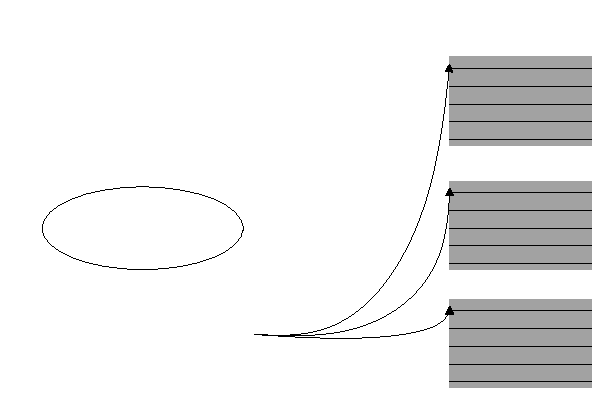
\includegraphics{figs/induced_operation_new.fig.eps}%
\end{picture}%
\setlength{\unitlength}{4144sp}%
%
\begingroup\makeatletter\ifx\SetFigFontNFSS\undefined%
\gdef\SetFigFontNFSS#1#2#3#4#5{%
  \reset@font\fontsize{#1}{#2pt}%
  \fontfamily{#3}\fontseries{#4}\fontshape{#5}%
  \selectfont}%
\fi\endgroup%
\begin{picture}(4392,2826)(31,-2053)
\put(271,-1951){\makebox(0,0)[lb]{\smash{{\SetFigFontNFSS{12}{14.4}{\familydefault}{\mddefault}{\updefault}{\color[rgb]{0,0,0}3. Create Function Evaluation}%
}}}}
\put(271,-1411){\makebox(0,0)[lb]{\smash{{\SetFigFontNFSS{12}{14.4}{\familydefault}{\mddefault}{\updefault}{\color[rgb]{0,0,0}1. Parse Function String}%
}}}}
\put(271,-1681){\makebox(0,0)[lb]{\smash{{\SetFigFontNFSS{12}{14.4}{\familydefault}{\mddefault}{\updefault}{\color[rgb]{0,0,0}2. Create Buffers}%
}}}}
\put(3331,-1321){\makebox(0,0)[lb]{\smash{{\SetFigFontNFSS{12}{14.4}{\familydefault}{\mddefault}{\updefault}{\color[rgb]{0,0,0}$C_3$}%
}}}}
\put(3331,-421){\makebox(0,0)[lb]{\smash{{\SetFigFontNFSS{12}{14.4}{\familydefault}{\mddefault}{\updefault}{\color[rgb]{0,0,0}$C_2$}%
}}}}
\put(361,-871){\makebox(0,0)[lb]{\smash{{\SetFigFontNFSS{10}{12.0}{\familydefault}{\mddefault}{\updefault}{\color[rgb]{0,0,0}$f(C_1,C_2,C_3)$}%
}}}}
\put(3331,524){\makebox(0,0)[lb]{\smash{{\SetFigFontNFSS{12}{14.4}{\familydefault}{\mddefault}{\updefault}{\color[rgb]{0,0,0}$C_1$}%
}}}}
\put( 46,614){\makebox(0,0)[lb]{\smash{{\SetFigFontNFSS{12}{14.4}{\familydefault}{\mddefault}{\updefault}{\color[rgb]{0,0,0}function: $(C_1+C_2)/(C_2-C_3)$}%
}}}}
\put( 46,389){\makebox(0,0)[lb]{\smash{{\SetFigFontNFSS{12}{14.4}{\familydefault}{\mddefault}{\updefault}{\color[rgb]{0,0,0}mapping: $C_1$=Channel 1}%
}}}}
\put(811,164){\makebox(0,0)[lb]{\smash{{\SetFigFontNFSS{12}{14.4}{\familydefault}{\mddefault}{\updefault}{\color[rgb]{0,0,0}$C_2$=Channel 2}%
}}}}
\put(811,-61){\makebox(0,0)[lb]{\smash{{\SetFigFontNFSS{12}{14.4}{\familydefault}{\mddefault}{\updefault}{\color[rgb]{0,0,0}$C_3$=Channel 3}%
}}}}
\end{picture}%
